\section{Analysis} \label{c:analysis}

Note that the code used to perform the analysis and generate all figures is publicly available on GitHub: github.com/Salahub/peremptory\_challenges.

\subsection{Visualization} \label{sec:visual}

First, consider a simple aggregate summary of the probability of removal by peremptory challenge by race in all data sets, shown in Table \ref{tab:margrace}.

\begin{table}[h!]
  \centering
  \caption[Strike Rate by Race]{\footnotesize The conditional probability of a venire member being struck peremptorily by venire member race across data sets. Note that the Philadelphia trial data only
    indicated black and non-black venire members and so only two numbers can be reported.} \label{tab:margrace}
  \begin{tabular}{|c|c c c|} \hline
    Data & Black & Other & White \\ \hline
    Sunshine & 0.23 & 0.24 & 0.25 \\
    Sunshine Capital & 0.22 & 0.27 & 0.27 \\
    Stubborn & 0.65 & 0.36 & 0.66 \\ 
    Philadelphia & 0.67 & \multicolumn{2}{c|}{0.68} \\ \hline
  \end{tabular}
\end{table}

These probabilities are different, but not greatly so. Indeed, the trend of higher probabilities for the removal of white jurors
across all data sets is perhaps counter-intuitive given the history of controversy in the United States. In any case, the small
magnitude of these differences suggests only a weak racial bias at the aggregate level.

This table also demonstrates some of the drawbacks of tables, the dominant method used to display the data throughout
\cite{JurySunshineProj}, \cite{StubbornLegacy}, and \cite{PerempChalMurder}. The table, while excellent at communicating specific
values, does not provide a sense of trends or patterns without careful engagement by the reader. A critical component of the
communication of any analysis and its comparison to others is the ability to quickly and effectively discern patterns in the data. Consequently, the ``mobile plot'' for visualizating the three-way relationships of categorical variables was
developed, with motivation from the hierarchy of visual perception of \cite{cleveland1987} and inspiration from \cite{VisualDisplayQuant}. It is used in Figure \ref{fig:racedefmob} to compare dispositions of venire members by their race and the defendant race for the Sunshine data.

\begin{figure}[!h]
  \centering
  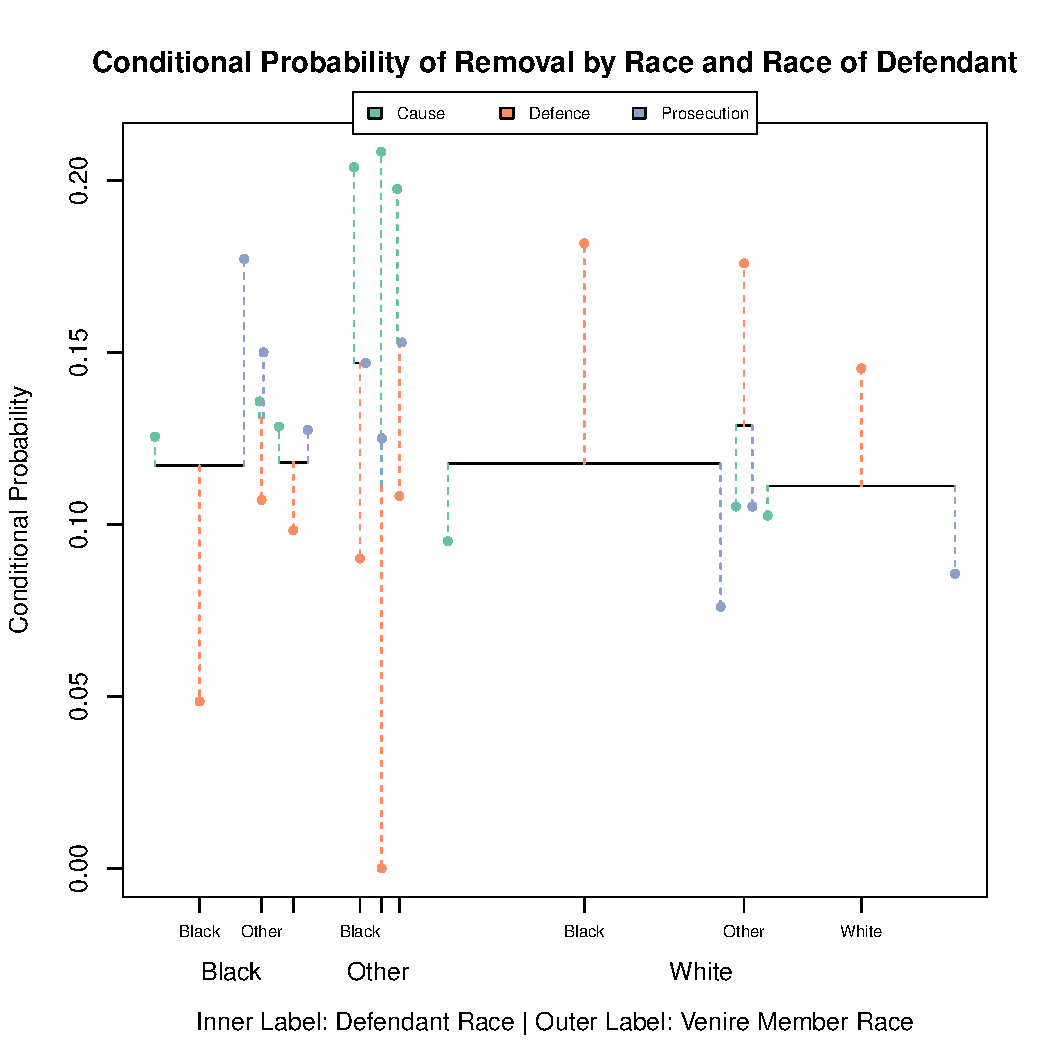
\includegraphics[width=0.7\textwidth]{RaceParCoord}
  \caption[The ``Mobile Plot'' of Strikes by Racial Combination (Sunshine)]{\footnotesize The conditional probability of strike disposition given the
    venire member and defendant race for the Sunshine data set. Expected values are represented by the horizontal black lines, and the observed values
    by the points at the end of the dotted lines. Each horizontal black line corresponds to a particular venire member
    and defendant race combination, with a length proportional to the number of venire members with that combination. The dashed
    vertical lines, coloured by challenge source, start at these horizontal lines and end at points which show the observed
    probability of a venire member being struck by the indicated party for the given racial combination.}
  \label{fig:racedefmob}
\end{figure}

First, a small explanation of the mobile plot. This mobile plot displays the relationship between three categorical variables:
venire member race, defendant race, and disposition (whether a venire member is struck and by whom). The vertical axis corresponds
to the conditional probability of a particular disposition given a racial combination. Racial combinations
are placed along the horizontal axis, and each combination corresponds to one horizontal black line in the plotting area. The
length of these lines is proportional to the number of venire members in the data with the corresponding racial combination, and
their vertical positions are the mean conditional probability of a
venire member being struck for that particular combination. The dashed vertical lines, coloured by disposition, start at this mean line and
extend to the observed conditional probability of the corresponding disposition for the relevant racial combination. As a
consequence, this plot can be viewed as a visualization of the test of a specific hypothesis:

\begin{equation}
  \label{eq:vishyp}
  D | D \neq \text{Kept}, R, E \sim Unif(\{\text{Prosecution
    Struck, Defence Struck, Struck with Cause}\})
\end{equation}

Where $D, R, E$ are random variables representing the disposition, venire member race, and defendant race, respectively. In words: the conditional distribution of the
disposition given the racial combination of a struck venire member is uniform. This implies that causal challenges, defence strikes, and prosecution strikes occur with the same probability for each
racial combination, though the rate may differ between racial combinations. Such a hypothesis allows for certain racial
combinations to experience a higher strike rate generally, but constrains the strike rate to be the same for all parties, which
would imply that all parties in the court pursue an identical strike strategy across all venire member and defendant race
combinations.

Clearly, Figure \ref{fig:racedefmob} casts some doubt on this hypothesis. While the horizontal black lines tell a very similar
story to Table \ref{tab:margrace}, with little variation between them except for in small population subsets, a number of other
striking patterns are visible. The first and most obvious of these is the main effect of venire member race. While the aggregate
removal rates do not seem to depend on the race of the venire member, it is clear that the defence and prosecution pursue
radically different strategies. The defence seems biased towards a jury composed of more racial minorities. All
orange points are below the horizontal lines for the black and other venire members, indicating these groups are less likely to be
struck by the defence than expected, while the points are above the lines for the white venire members, indicating a higher than
expected probability of a defence strike. The prosecution seems to mirror this tendency, striking the
white venire members at a lower rate than expected and the black venire members more often than expected. Challenges with cause
seem to show less deviation from expectation for the black and white venire members, and always deviate from expectation
in the same direction as the prosecution.

The addition of defendant races shows another interesting trend. It would seem that the aforementioned tendencies of the
prosecution and defence are strongest for black defendants, which have the greatest departures of the conditional probabilities
from the expectation. The defence and prosecution seem to have slightly more similar habits when the defendant is white, despite
their opposite tendencies in all cases. Finally, it would seem that the challenges with cause follow patterns similar to the
prosecution, as the points representing the conditional probability of a venire member being removed with cause are always on the
same side of the expected line, an event which would occur with probability $2^{-9} \approx 0.002$ under the hypothesis of
independent uniform strike rates. Section \ref{sec:mods} discusses the agreement of these two strike tendencies further.

\begin{figure}[h!]
  \centering
  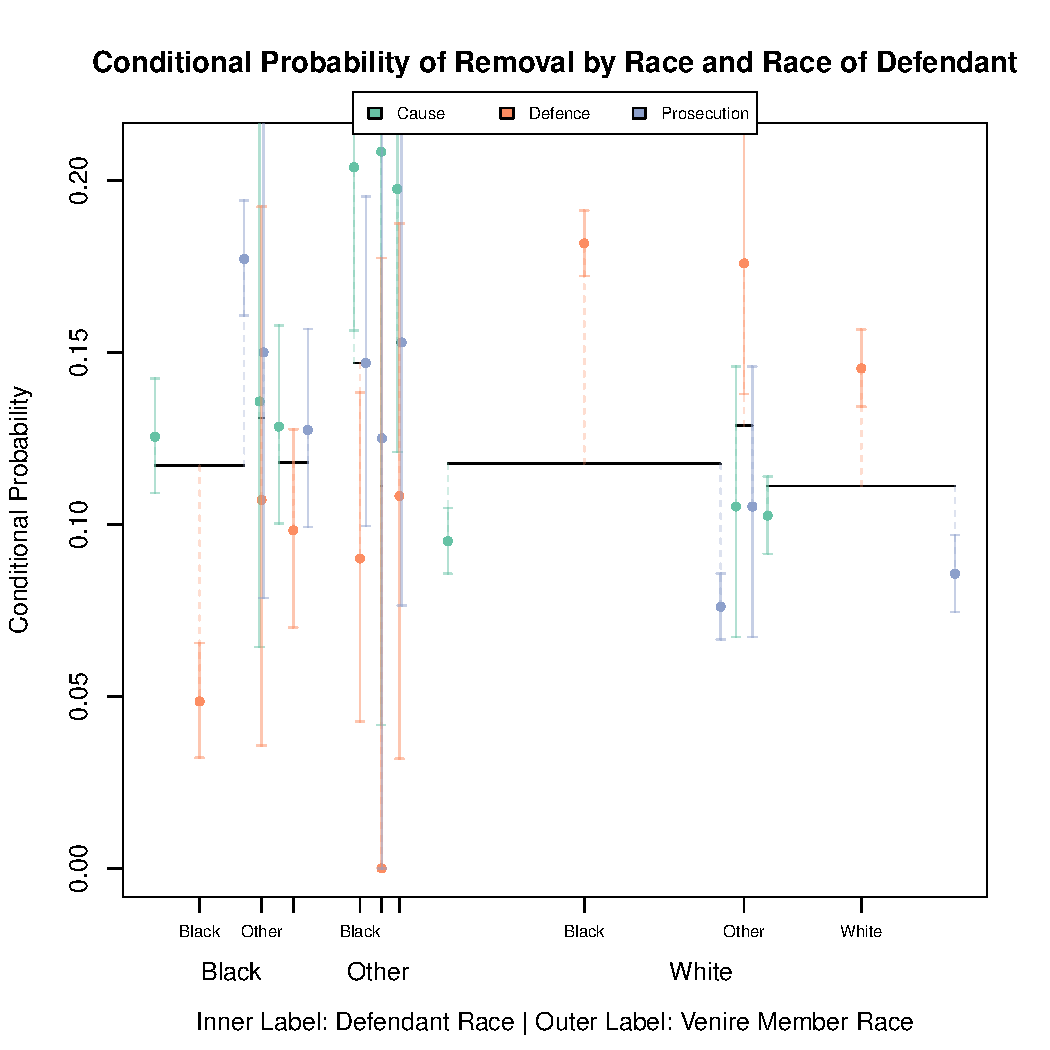
\includegraphics[width=0.7\textwidth]{RaceDefCI}
  \caption[Strikes by Racial Combination with Confidence
  Intervals (Sunsine)]{\footnotesize The plot of conditional strike probability by racial
    combination from Figure \ref{fig:racedefmob} with confidence intervals added. Note that many of the seemingly striking departures seen are
    insignificant when these confidence intervals are applied,
    especially for races other than black and white.}
  \label{fig:racedefci}
\end{figure}

While Figure \ref{fig:racedefmob} is quite suggestive, the widths of certain horizontal black lines, in particular those for
venire members with a race other than white or black, suggest that some of the more extreme tendencies are simply a result
of the well-known greater variation of samples with small sizes. In order to see the true nature of the noted departures some
incorporation of the expected variation is required. This is accomplished by the addition of
approximate 95\% simultaneous multinomial confidence intervals using the \texttt{MultinomialCI} package in R, which implements
simultaneous confidence intervals for multinomial proportions following the method presented in \cite{sison1995}. These confidence
intervals can be seen in Figure \ref{fig:racedefci}.

As suspected, some of the results for the smaller sample sizes do not seem to be significant. However, the results for the larger groups,
in particular for white venire members or black defendants, are significant. It should be noted that these simultaneous
confidence intervals do not constitute a proper statistical test of the impact of race, they are rather a way of visually
providing a viewer some sense of the expected variability in the data over repeated sampling. More rigorous testing requires
controlling for the impact of confounding factors, as done by the modelling in Section \ref{sec:mods}.

\subsubsection{In the Stubborn and Philadelphia Data}

\begin{figure}[h!]
  \centering
  \begin{subfigure}{0.32\textwidth}
    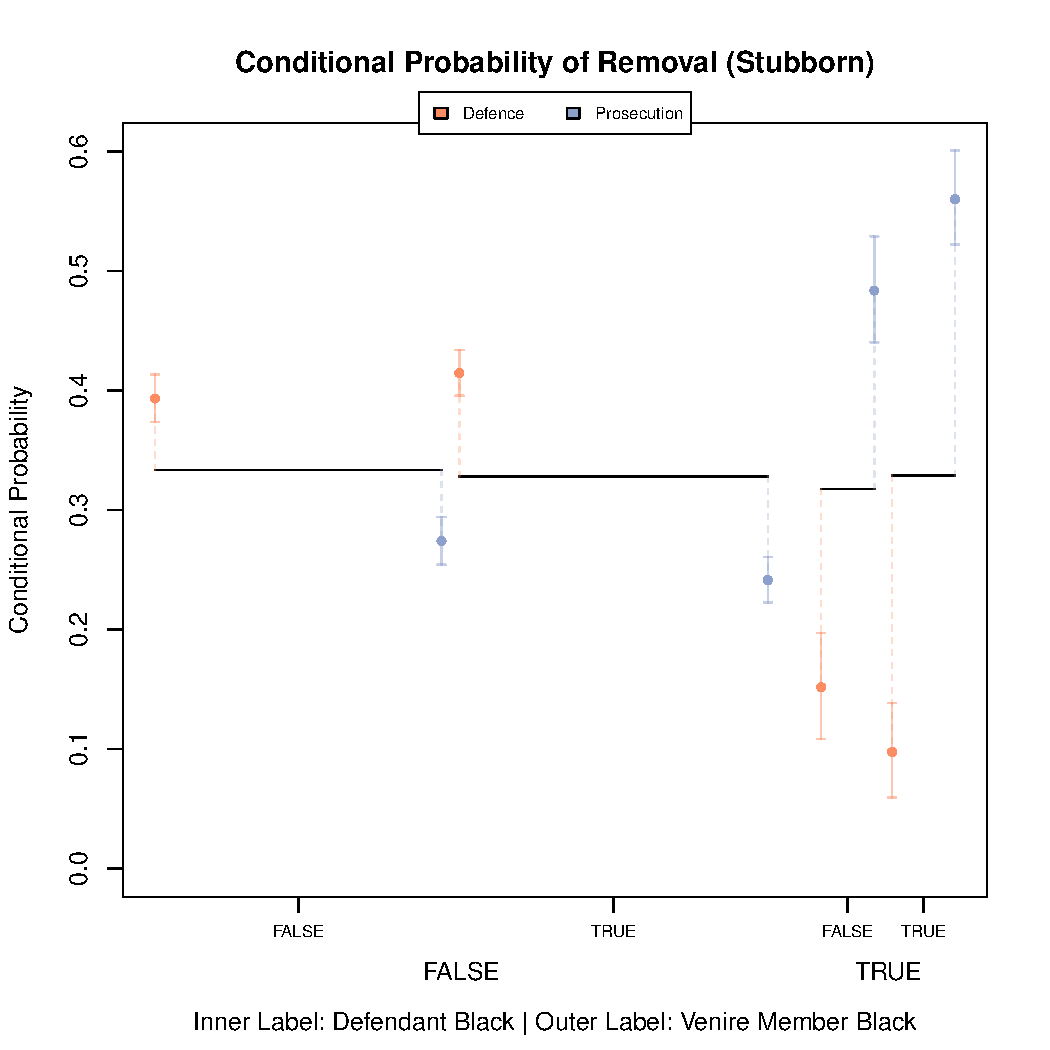
\includegraphics[scale = 0.32]{StubbornCompPlot}
    \caption{\footnotesize Stubborn strike pattern}
    \label{fig:stubcomp}
  \end{subfigure}
  ~
  \begin{subfigure}{0.32\textwidth}
    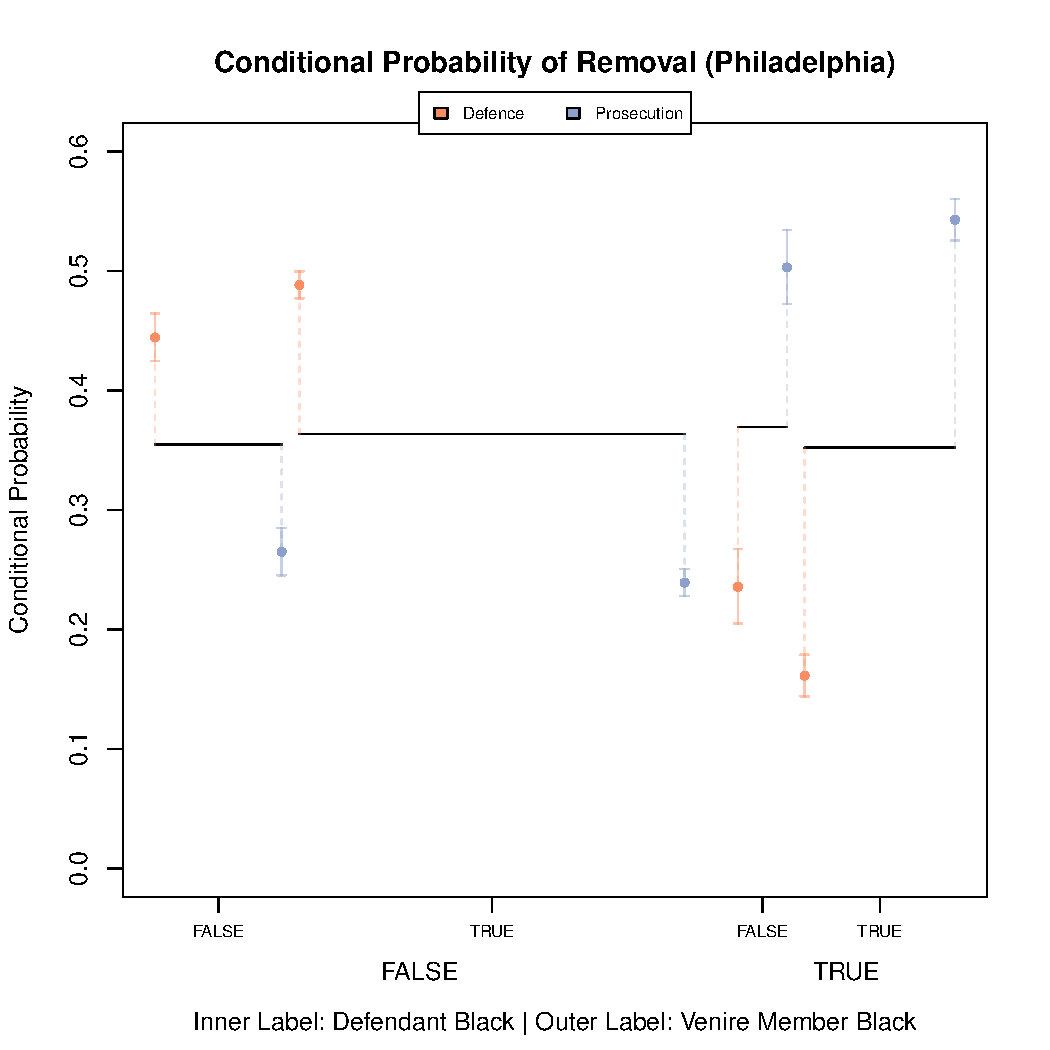
\includegraphics[scale = 0.32]{PhillyCompPlot}
    \caption{\footnotesize Philadelphia strike pattern}
    \label{fig:philcomp}
  \end{subfigure}
  ~
  \begin{subfigure}{0.32\textwidth}
    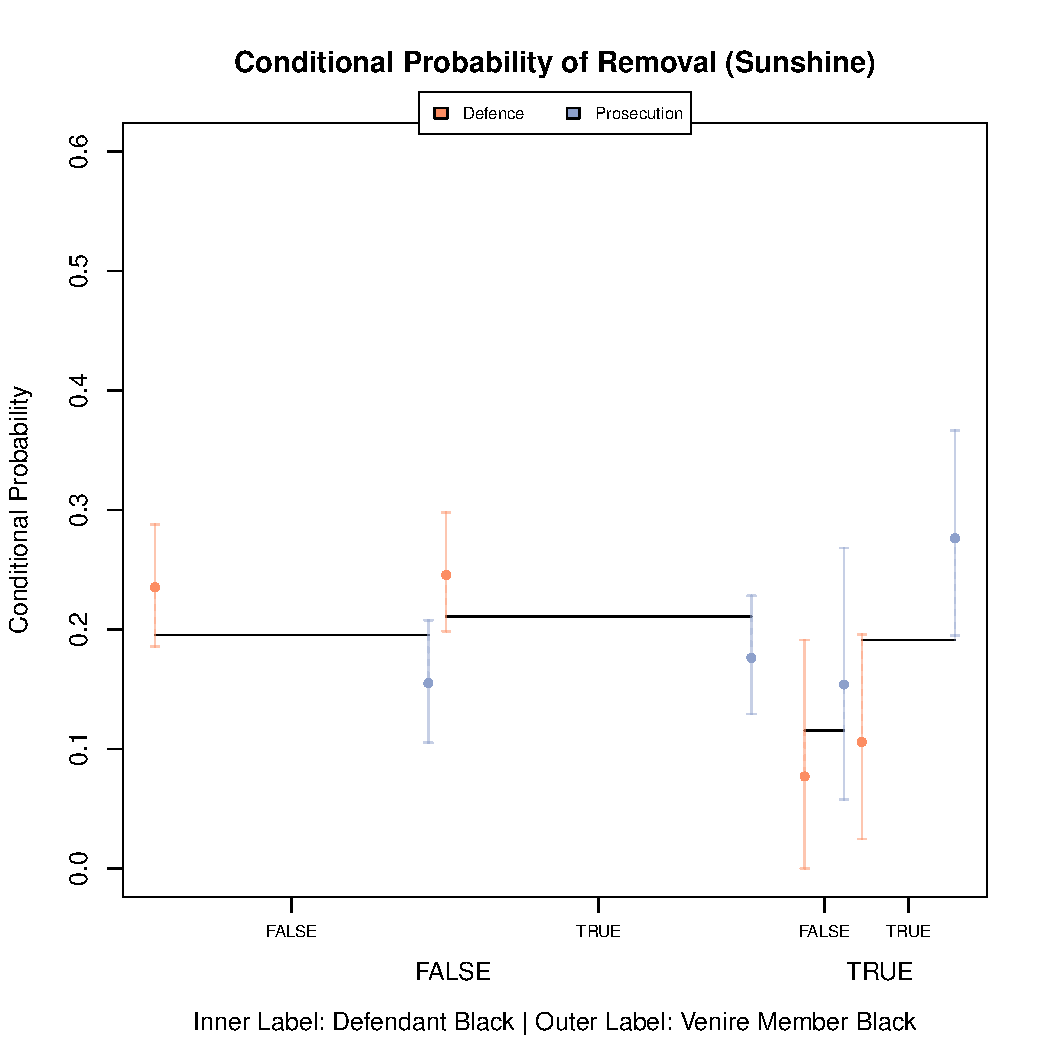
\includegraphics[scale=0.32]{SunshineCompPlot}
    \caption{\footnotesize Sunshine strike patternx}
    \label{fig:suncomp}
  \end{subfigure}
  \caption[Strikes by Racial Combination (All Capital Trial Data)]
  {\footnotesize The conditional probability of defence and prosecution peremptory challenge by race across all
    capital trials in all data sets. The pattern, though sometimes different in magnitude, is quite consistent across the three,
    despite the significant differences in the respective study sample universes.}
  \label{fig:racedefalldata}
\end{figure}

Already the utility of the mobile plot, and visualizations of the data in general, should be clear. A wealth of information is
displayed very simply in Figure \ref{fig:racedefci}. However, the real power of this plot comes with the ability to quickly
compare different data sets. Consider, for example, comparing all three data sets
using Table \ref{tab:margrace}. In order to compare, the rows for each data set must be viewed and the numbers
committed to memory before the reader moves to the appropriate row to compare values. While the simple four row and three column
structure of this particular table make this rather straightforward,
it becomes more difficult as the table grows
in complexity. Compare this with a cursory glance at Figure \ref{fig:racedefalldata}, which makes the similarities of the data
sets immediately clear. Note that the restricted study sample universes of the Philadelphia and Stubborn data make these plots considerably different than Figure \ref{fig:racedefci}.

Despite the very different study populations of these three data sets, all display similar patterns, with only the
magnitudes of the strike rates differing. The mobile plot format reveals several interesting aspects. The similar level of all black lines within each plot shows that in each data set, the aggregate probability of removal is
similar across racial combinations, as was implied by Table \ref{tab:margrace}. However, these aggregate similarities
hide the vastly and consistently different strategies of the defence and prosecution across all data sets. The defence has a
tendency to retain black venire members, striking them at a lower rate
than the other venire members, while the
prosecution shows a pattern which mirrors that of the defence,
removing more black venire members and fewer other venire members. In
all data sets the gap between these probabilities and the expected strike rates are greatest for the black venire members in cases
with black defendants.

It should be noted that the Sunshine data set looks most unique of the three, and this may be a result of the sampling method. While
the Philadelphia data and Stubborn data both collected data which included multiple years and selected capital cases only, the Sunshine data was restricted to
trials which occurred in 2011 and collected all cases. This small sample is the reason for the large confidence intervals present in Figure
\ref{fig:suncomp}. This does not explain the overall lower strike rate observed in the capital trials in the Sunshine data, which is also
visible in Table \ref{tab:margrace}. This departure may be of interest for future investigation.

\subsection{Modelling} \label{sec:mods}

Of course, it would be incorrect to conclude immediately that the cause of the racial patterns observed across these data sets is
race itself. There may be a plethora of attitudes associated with race that could serve as legitimate cause for a peremptory
challenge, as noted by Justice Byron R. White in the majority opinion in \textit{Swain v. Alabama} [\cite{swainvalabama}].

Without detailed transcripts detailing voire dire, it cannot be known if the aggregate pattern of removal is the result of racially based strikes, or whether the lawyers
determined valid reasons for a peremptory challenge during the voir dire process related to race. For example, if
defence attorneys reasonably assumed that deference to authority would make a venire member insurmountably predisposed to reject
their arguments about mishandling of evidence by police, this would be reasonable grounds for
peremptory challenge. If such opinions were distributed heterogeneously by race, the aggregate pattern may appear to reflect
racially-based decision making by the defence attorneys despite the
true explanation being legitimate and non-racial. Such ``ideological imbalance'' in political affiliation was noted in \cite{revesz2016}.

Answering this question precisely requires that all available confounding factors be controlled. While such controlled modelling has already been completed for \cite{StubbornLegacy} and \cite{PerempChalMurder}, no such modelling has been completed for the much richer and larger Jury Sunshine data set. The design of the mobile plot further motivates such multivariable regression by suggesting a particular form of model: the multinomial logistic regression model.

\subsubsection{Multinomial Logistic Regression}

Though the above results in the Sunshine data set may be suggestive, refining the estimates for the impact of race on the
probability of rejection and controlling for the myriad of possible confounding factors motivated the fitting of multiple
models. This is helped by the nature of the mobile plots used in
Figure \ref{fig:racedefmob} and elsewhere. The mobile plot displays the
conditional distribution of a categorical variable with multiple levels, which suggests modelling with a conditional multinomial
distribution. Consequently, fitting multinomial log-linear regression, or equivalently a Poisson regression [\cite{baker1994}; \cite{lang1996}], seemed a natural choice. The specific implementation of multinomial regression utilized is the
\texttt{multinom} function in the \texttt{nnet} package in R, which implements a method of fitting multinomial models discussed
in \cite{nnet}.

For all models, the pivot outcome chosen was the probability of a
venire member sitting on the final jury, in other words the probability their disposition was coded as \texttt{Kept}. Coefficients were
then estimated using treatment contrasts with a black female venire member with Democrat voting tendencies in a case with a black female
defendant used as the reference treatment.

While the choice of race, gender, and political affiliation for the reference level was not deliberate, the choice of pivot
outcome, that of a venire member being kept, was made in order to make the visualizations constructed using the coefficients easy to compare to previous visualizations. Previous visualizations, including the mobile plots, have displayed the
conditional probabilities of removal with cause and strikes by defence and prosecution, and if any were used as the pivot their
coefficient estimates would be hidden as the intercept.

The mobile plots created in \ref{sec:visual} also suggest that an interaction between race and
defendant race is relevant in modelling the conditional probability of venire member rejection. This motivated a model of all main effects and an interaction effect between the race of the venire member and that of the defendant, called the full model. To test this interaction and the impact of venire member race in the presence of all other variables, models excluding this interaction and excluding venire member race were also fit, called reduced models 1 and 2 respectively. The deviance residuals of all three models were used to perform ANOVA tests comparing \ref{eq:noraceintmod} and \ref{eq:novmmod} to \ref{eq:fullmod}. These can be see in Table \ref{tab:modcomp}, which compares the deviances of the different models sequentially when fit to the Jury Sunshine Data.

\begin{table}[h!]
  \centering
  \caption[Nested ANOVA Table Demonstrating the Importance of
  Race]{\footnotesize Comparison of models, displaying the residual deviance, residual degrees of freedom, differences, and p-values of these
    differences for adjacent models.}
  \label{tab:modcomp}
  \begin{tabular}{|c|c|c|c|c|} \hline
    Model & Residual df & Residual Deviance & Difference & $P(\chi^2)$ \\ \hline
    Reduced Model 2 & 55527 & 39496 &  &  \\
    Reduced Model 1 & 55521 & 39087 & 405 & ~0 \\
    Full Model & 55509 & 39023 & 67 & 1.4e-9 \\ \hline
  \end{tabular}
\end{table}

Even when controlling for defendant characteristics and the venire member's political affiliation and sex, the race of the venire
member and its interaction with the defendant race are both highly significant at the $\alpha = 0.05$ level. This suggests that
the rejection of venire members is, at least in part, based on their racial characteristics. Note that the residual deviance values indicate that this model
is underdispersed, implying that the significant test results gained
are conservative.

Due to its significance compared to the other models, \ref{eq:fullmod} was taken as the final model to estimate the race effects
with precision. Inspired by \cite{dotwhisker}, a custom dot and whisker plot was generated to display these coefficients. This plot displays the coefficient estimates as points in the centre of a line, the endpoints of which
give the associated confidence intervals. A vertical line is placed at zero to provide a reference for the sign and significance
of different parameters. Modifying this concept to suit the multinomial regression data was simple, as it only required grouping
the different possible outcomes for each parameter spatially.  The estimated coefficients for the different effects and their approximate 95\% confidence intervals, calculated using the standard errors of the coefficients and using a normal assumption, are displayed using this modified dot-whisker plot in Figure \ref{fig:modallcoef}.

\begin{figure}[h!]
  \centering
  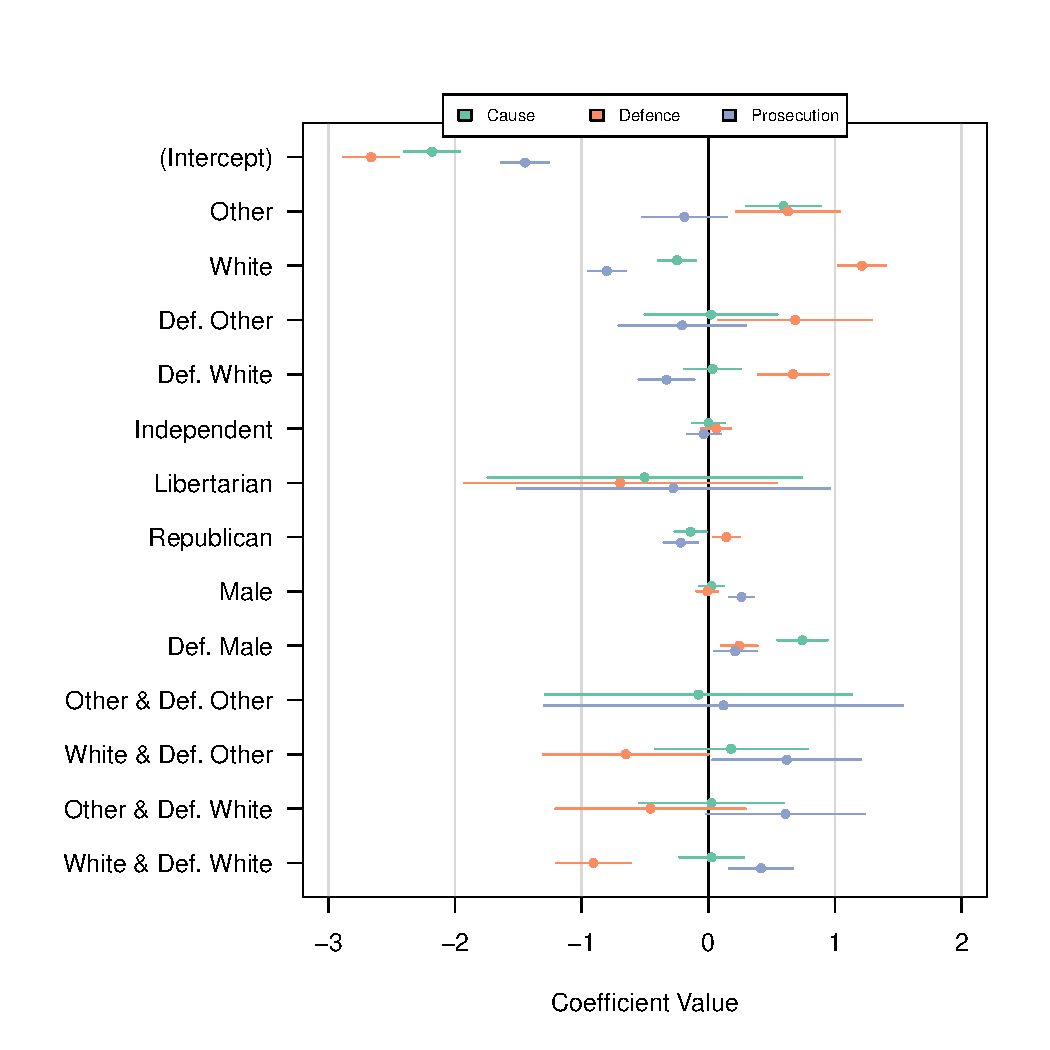
\includegraphics[scale=0.7]{AllModCoef}
  \caption[All Model Coefficients]{\footnotesize Model coefficients from the full model, \ref{eq:fullmod}, displayed using
    a dot-whisker plot. The lines indicate the confidence intervals while the central points indicate the point estimates of
    coefficients.}
  \label{fig:modallcoef}
\end{figure}

%\begin{figure}[h!]
%  \centering
%  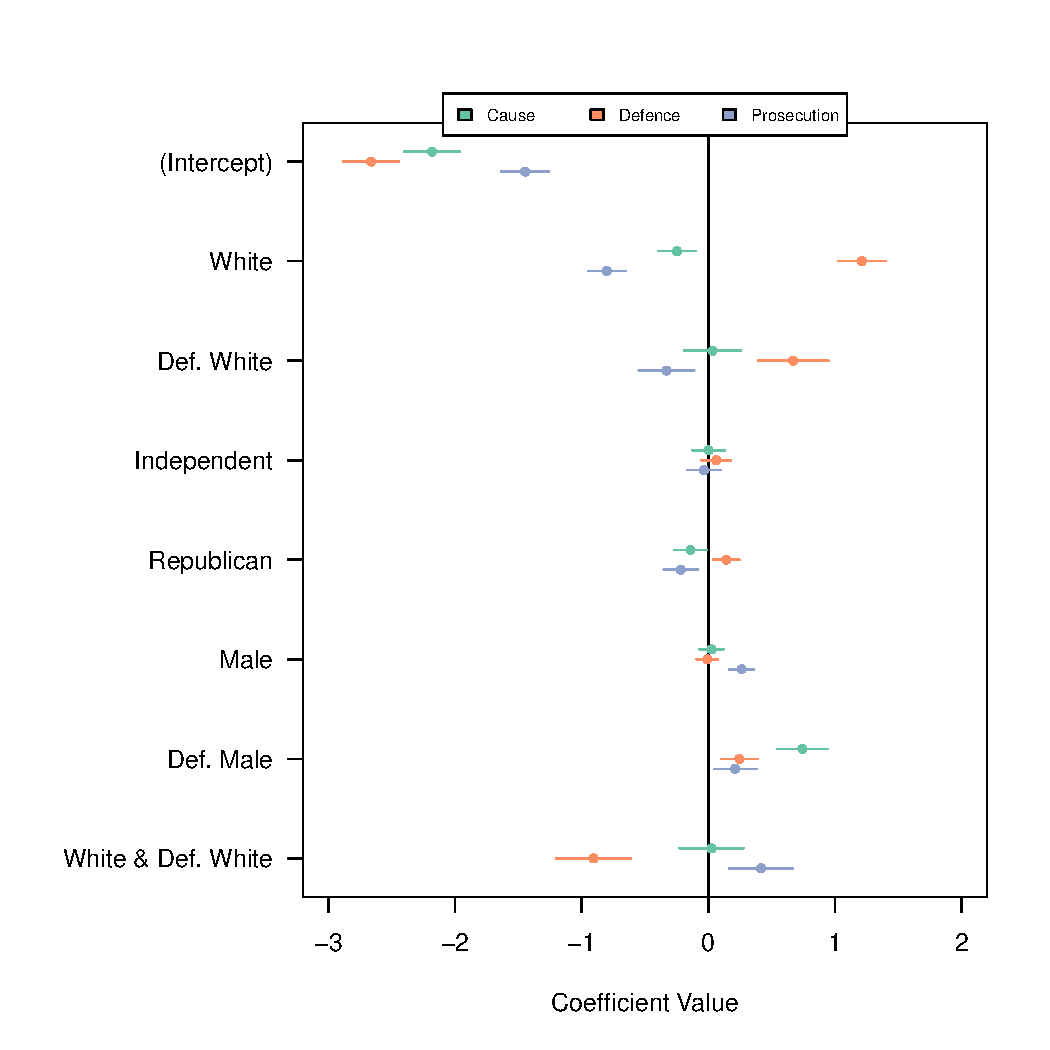
\includegraphics[scale=0.7]{SelectModCoef}
%  \caption[Select Model Coefficients]{\footnotesize Select model coefficients from the full model displayed using a dot-whisker
%    plot. The lines indicate the confidence intervals while the central points indicate the point estimates of coefficients.}
%  \label{fig:modselcoef}
%\end{figure}

The first feature of this plot to notice is the position of the coefficient estimates relative to the black line at zero. This
indicates the sign of the coefficient, positive if the point is to the right and negative if it is to the left. A positive sign
indicates that the factor corresponding to the coefficient increases the probability of a venire member being struck by a particular party and a negative sign indicates that the presence of said factor decreases the
probability of a venire member being struck. The pattern of positive and negative values suggests the uncontrolled patterns
noticed in the mobile plots were not the result of confounding.

First, take a broad overview of the patterns. The variables which show the greatest significance and the characteristic
oppositional tendencies of the prosecution and defence are all race variables. The effect of a white venire member, white
defendant, and their interaction all display significant, and opposite, tendencies for these two oppositional parties. Moreover,
the magnitude of the defence coefficients is always greater than the prosecution for the race variables. This suggests that the
defence probability to strike is affected far more by race variables than the prosecution probability to strike. To put this more
simply, the defence is more sensitive to the racial aspects of the trial in general.

A quick survey of the prosecution and cause coefficients shows far less agreement than seemed apparent in the mobile
plots. Scanning from the top to the bottom, the cause coefficients match the prosecution for a few groups, but are generally quite 
different and are often more similar to the defence than the prosecution. The suggestive pattern of matching prosecution strikes
and causal strikes viewed in \ref{sec:impactrace} vanishes when controls are placed on possible confounders. In general, the cause strike
coefficients are lower in magnitude than both the prosecution and defence, with the notable exception of the effect for male
defendants, where it is significantly greater than both.

In order to examine patterns in more detail some important differentiation is necessary between the intercept values and the other
coefficients. As with all linear models, the intercept values provide a locational measure. That is to say, the intercepts provide
the base level upon which the coefficients act. Consequently, the
negative values of the intercept for all striking parties is to
be expected. In the Sunshine data more venire members were kept than rejected, as can be seen in Tables \ref{tab:margrace} and
\ref{tab:rejbounds}, and so the intercept, which gives the log odds ratio of each strike outcome to the venire member being kept,
would naturally be negative for all parties.

The more important feature to note for this intercept is the large
difference between the different striking parties, without
overlapping confidence intervals. These suggest that all three parties behave differently in the reference group, which
consists of a female, black, Democrat venire member in a case with a female, black defendant. Crucially, the defence intercept is
far lower than the prosecution, matching what was observed in Figure \ref{fig:racedefmob}, where the lowest defence strike
probability occurred for black venire members in cases with black
defendants. Also visible in Figure \ref{fig:racedefmob} is an increase in
defence strike probability and decrease in prosecution strike probability for a white defendant with a black or other venire
member. This pattern is reflected perfectly in the positive defence coefficient and negative prosecution coefficient for white
defendants.

The coefficients for white venire members also match the expectations of Figure \ref{fig:racedefmob}. The defence attains its
largest positive coefficient for this group and the prosecution is largest negative value. The dominant effect of venire member
race visible throughout the mobile plots in \ref{sec:otherfact} and \ref{sec:impactrace} is reflected by the dominance of the
magnitudes of the coefficients for white venire members relative to the reference black venire members. The defence is much more
likely to reject a white venire member and the prosecution much less likely.

Slightly attenuating this pattern is the interaction effect between a white defendant and a white venire member. For this specific
combination, the defence is less likely to reject than for a white venire member with a black or other defendant, while the
prosecution is more likely to reject. Both of these trends seem to be significant based on the plotted confidence
intervals. Combine this observation with the almost mirrored pattern for a white defendant with a black venire member (given by
the white defendant coefficient), and a more nuanced strategy becomes clear. While the prosecution dominantly rejects black venire
members and the defence dominantly rejects white venire members, they are also sensitive to possible racial matches. The defence
pattern is consistent with a strategy which aims to partially select for venire members which have the same race as the defendant,
while the prosecution has the opposite pattern.

This pattern is precisely the problematic behaviour which was implied by the individuals that viewed \textit{R. v. Stanley} as a
travesty. While the data here \textit{cannot} reveal anything about that \textit{specific} trial, or indeed about the exercise of
peremptory challenges in Canada generally. That such a pattern is clearly present in the data will no doubt feel vindicating for
those still musing on \textit{R. v. Stanley}'s perceived injustice.

Such racial patterns in the prosecution and the defence dominate all other effects. The political effect is minor, though
consistent with the hypothesis put forward by \cite{revesz2016}, with a preference for Republicans by the prosecution and a
preference for Democrats by the defence. Interestingly, all parties
seem to have an increased strike probability for male venire
members, suggesting a universal preference for female venire members on the jury. One would hope that this pattern is for some
other reason than anything listed on pages 152-153 of \cite{vandykejurysel} and reproduced here in \ref{sec:polaff}. While no
detailed explanation is forthcoming for this pattern in the presence of racial and political affiliation controls, it would
certainly be an interesting avenue for further research, as the exercise of peremptory challenges based purely on gender is also
protected by \textit{J.E.B. v. Alabama} [\cite{jebvalabama}].

\subsection{Trial Level Summary} \label{sec:casesum}

While \cite{JurySunshineProj} reported a great deal of aggregate statistics about the venire members themselves, one piece of
investigation which was lacking was an analysis which viewed the trends for cases, rather than simply for
individual venire members. As it cannot be known why a particular venire member is struck, and viewing their aggregate
statistics tells us nothing about how different strikes relate to each other, it is possible the aggregate patterns are the result
of some effect which is not due to persistent bias across trials.

By aggregating the venire members by trial and viewing the demographic trends in strikes and behaviour at this level,
detailed insight into the impact of challenges at a more relevant scale is gleaned. Aggregation to the trial level naturally controls for differences created by judges, lawyers, and cases by grouping together venire members exposed to the same values for these variables. This particular perspective of the data has also not been explored by any other studies
known to the author.

\subsubsection{Estimating Struck Juror Counts} \label{subsec:struckjur}

One gap which was present in the Sunshine data was the total count of defence and prosecution removals for each trial. This
variable is of minor importance for modelling the individual venire
members, but it is of major interest when viewing the trials
themselves. While counts of these strikes were provided in the data, there were many missing values, or values inconsistent with
the number of associated venire members in the data. For example, many of the recorded values in these columns were zero even when
venire members associated with that trial were marked as struck.

To remedy this, a number of variables were generated for each trial. Primarily, these variables were counts of the number of
venire members with particular characteristics which were struck by both the prosecution and defence in the trial. For example the
variable \texttt{DefRem.Race.Black} provided the count of black venire members struck by the defence for a specific trial. To
provide an estimate of the number of venire members struck by each
party, these counts were summed for one particular
variable, typically gender. The sum was then compared to the recorded value for that party's removed count. The greater of the two
values was kept as an estimated count to be used in analysis. For both the prosecution and the defence, about 80\% of the sum and
recorded values matched exactly and about 18\% of the recorded values were less than the sum. This suggests some incompleteness
for the remaining 2--4\% of the data.

\subsubsection{Visualizing the Racial Trends} \label{subsec:vistrend}

Motivated by the plots in the \texttt{extracat} package in R [\cite{extracat}], in particular the \texttt{rmb} plot, a
positional proportion plot, called here the ``positional boxplot,'' was developed to display the strike tendencies across
trials. The data for each trial consists of categorical variables and two integer counts corresponding to the estimated defence
and prosecution strike counts described in \ref{subsec:struckjur}. The positional boxplot was developed to investigate the
relationship between the strike patterns of both parties and the defendant race.

\begin{figure}[h!]
  \centering
  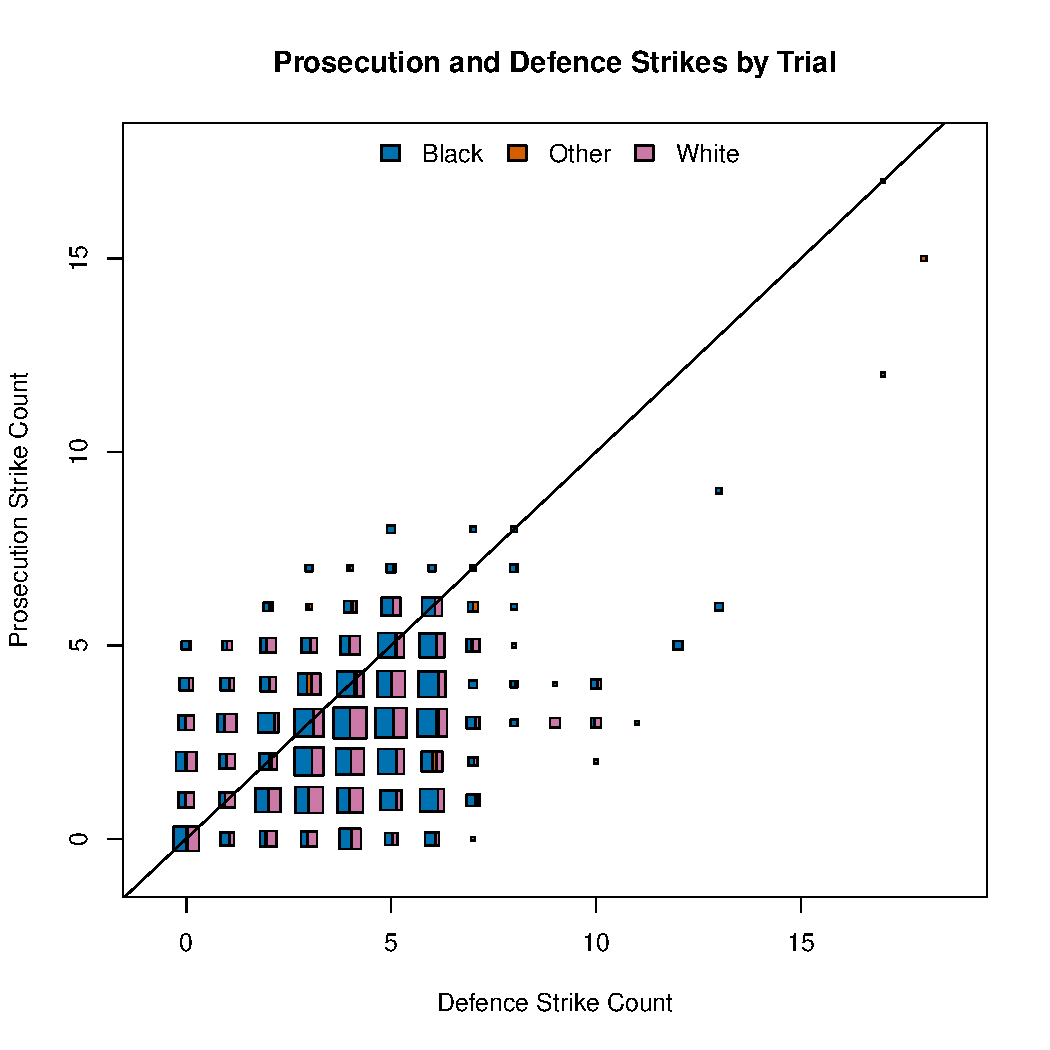
\includegraphics[scale=0.7]{DefProStrikesTrial}
  \caption[Prosecution and Defence Strikes by Trial]{\footnotesize The positional boxplot of strikes by race of defendant for the
    Sunshine data. There does not seem to be a dependence of strike counts on the defendant race, the boxes look similar across
    the entire plot.}
  \label{fig:trialprodef}
\end{figure}

Therefore, the positional boxplot is designed to visualize the conditional distribution of a categorical variable given two
integer count variables. Each observation consists of a level of a categorical variable and two counts. Across the whole data,
there may be occurrences of identical values for the two counts. At each unique combination of integer counts observed, a box is
placed with an area proportional to the number of observations with that specific combination. Each box is then subdivided
horizontally such that the width of each subdivision is proportional to the corresponding count of each level of the categorical
variable that occurs with that specific integer combination.

Figure \ref{fig:trialprodef} displays a positional boxplot of defendant race to prosecution and defence estimated strike
counts. While the internal box patterns look rather similar everywhere, split somewhat evenly between black and white defendants,
their areas are quite revealing. In the aggregate examination of the data, it was clear that the defence had an overall higher
strike rate than the prosecution, this effect can be viewed clearly in Figure \ref{fig:gengen} where the defence has a higher
strike rate across all gender combinations. What was not clear was whether this pattern reflected the typical pattern at the
individual trial level or was rather due outlier cases with abundant defence strikes. The areas of the boxes in Figure
\ref{fig:trialprodef} indicate clearly that the defence typically uses more peremptory challenges than the prosecution in each
trial.

This plot may be somewhat misleading, however, as it fails to account for
the number of black and white venire members presented to the court in each of the trials. These numbers are very different, as can be seen by the
lengths of the horizontal black lines in Figure \ref{fig:racedefmob}. A sizeable majority of the venire members are
white. Luckily, with trial aggregated data, the raw strike counts can be normalized into proportions. The resulting scatterplots
of these proportions by trial are displayed in Figure \ref{fig:defproprop}.

\begin{figure}[h!]
  \centering
  \begin{subfigure}{0.45\textwidth}
    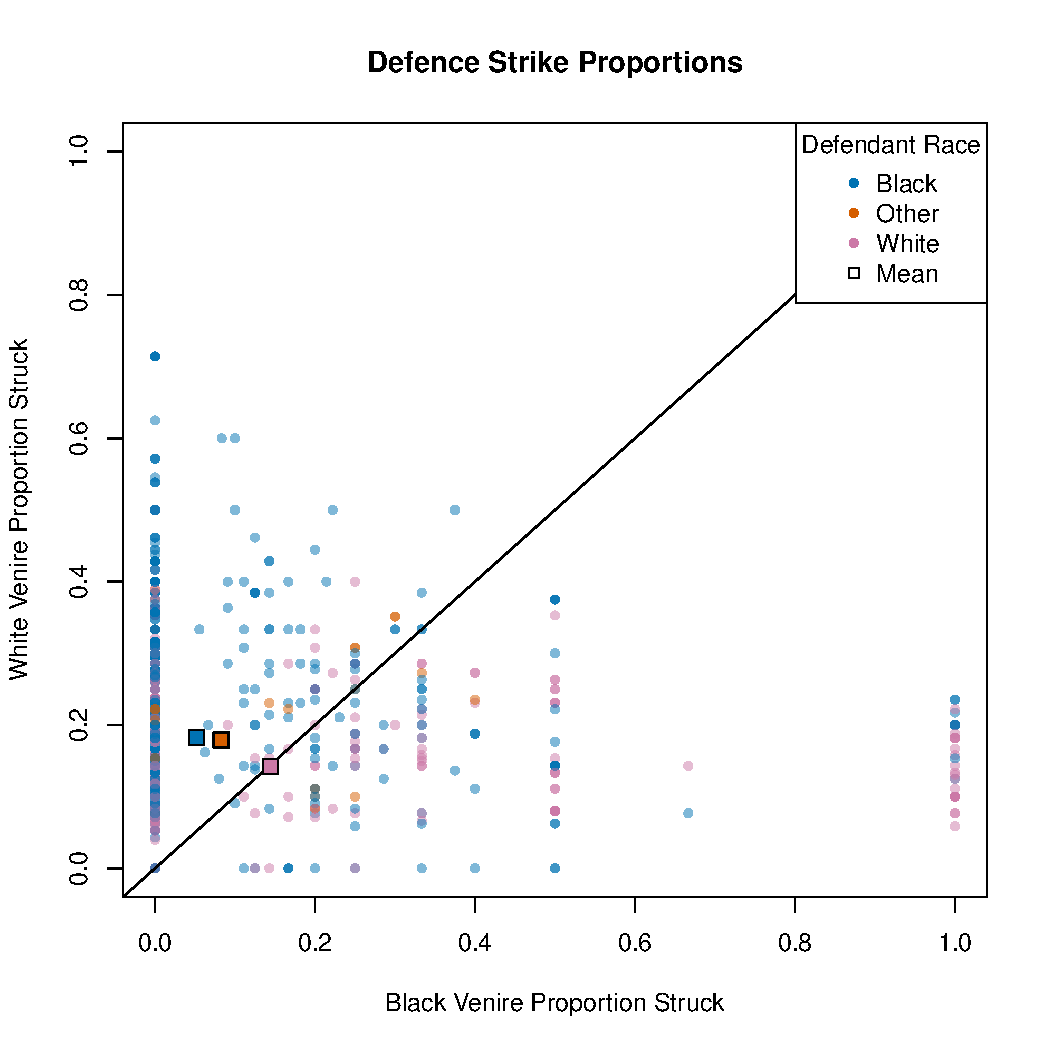
\includegraphics[scale = 0.45]{DefStrProp}
    \caption{\footnotesize Defence proportion venire removed}
    \label{fig:defraceprop}
  \end{subfigure}
  ~
  \begin{subfigure}{0.45\textwidth}
    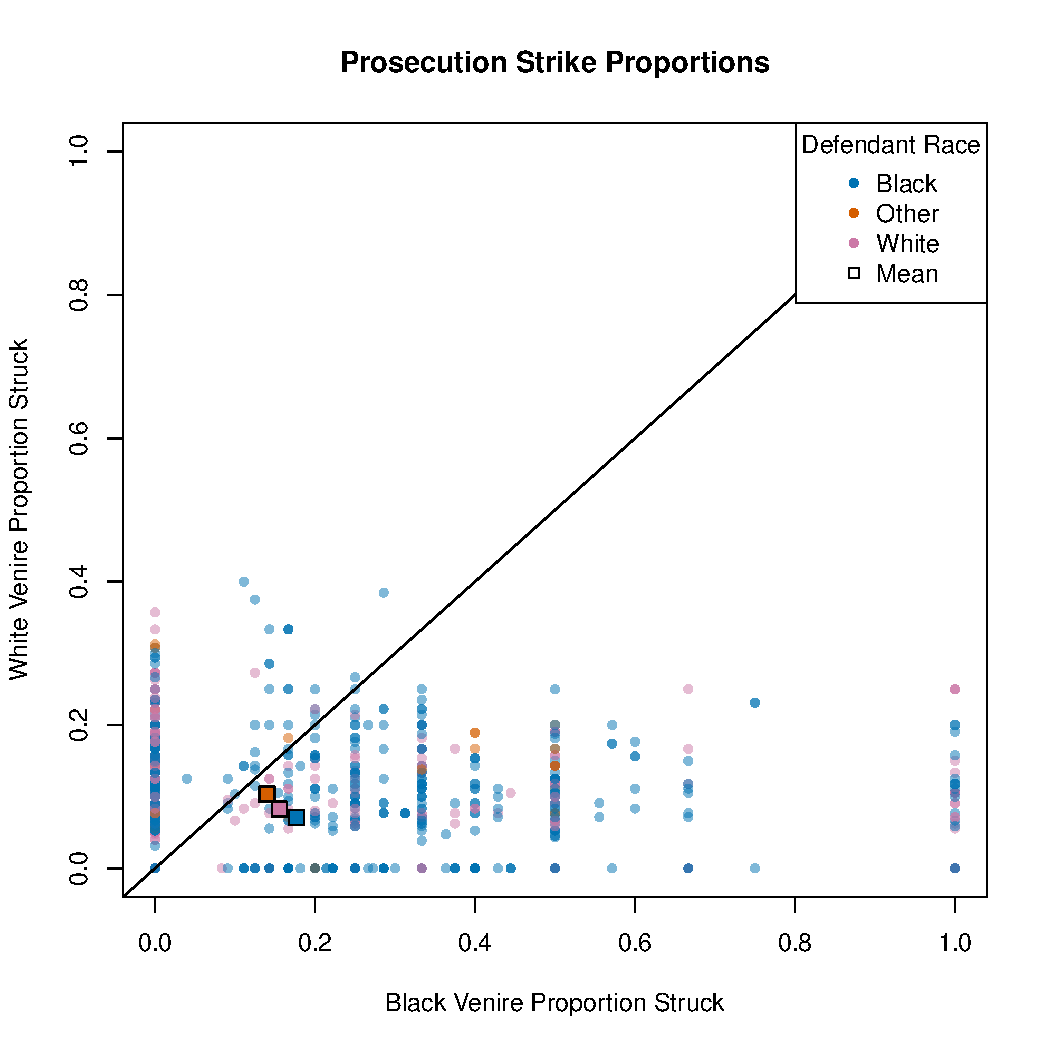
\includegraphics[scale = 0.45]{ProStrProp}
    \caption{\footnotesize Prosecution proportion venire removed}
    \label{fig:proraceprop}
  \end{subfigure}
  \caption[Racial Strike Proportions by Party]
  {\footnotesize Scatterplot of venire proportion removed by race for both the defence and prosecution.}
  \label{fig:defproprop}
\end{figure}

Here, the prosecution and defence biases are much more clear. The prosecution never strikes more than 40\% of white venire members
presented, and on average strikes a greater proportion of the black venire than the white venire. The defence, in contrast,
regularly strikes more than 40\% of the white venire, and on average strikes a greater proportion of the white venire members than
the black venire members. This reinforces the aggregate observations made in \ref{sec:mods}, indicating that these mechanics
operate on the individual trial level, and not just over all trials. Additionally, the high variation visible in Figure
\ref{fig:defproprop} suggests that the aggregate patterns described in \ref{sec:mods} are not followed by all defence or
prosecution lawyers, merely on average.

While these differences are intriguing, the far more interesting observation that can be gleaned from these plots is the
fundamental difference in inclusion of minority and majority groups in jury formation. The aggregate statistics indicate that the
black venire members are a minority, and Figure \ref{fig:defproprop} suggests that as a consequence, it is common that a majority
or all of the potential black jurors will be removed by peremptory
challenge. Such an occurrence is not observed in this data for the
majority white venire members, suggesting the complete removal of
white venire members is incredibly rare, if not impossible. While in many trials all black venire members were struck, in not a single trial was
every white venire member struck. This suggests that if one had a strategy of keeping minorities off of juries, the peremptory
challenge system would make this task easier. Such an observation is obvious in theory, but it is no less impactful to see it
emerge from the data.

Of course, more critical to this issue is the underrepresentation of marginalized groups in jury venires, as noted by \cite{vandykejurysel}. Their reduced representation and small numbers at the time of jury selection allows for their complete exclusion in a large number of trials. This is due to a combination of factors including the method of jury summons and the compensation given to jurors, and cannot be solved by the removal of peremptory challenges alone.
